\documentclass{beamer}
\usepackage{tikz}
\begin{document}
	\begin{frame}
		\frametitle{Introduction}
		\framesubtitle{Background and motivation}
		\begin{figure}[!h]
			\centering
			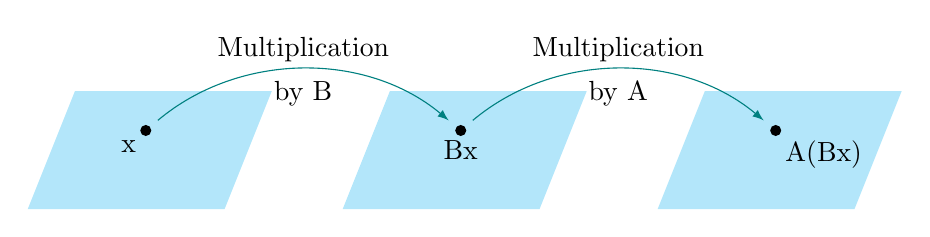
\begin{tikzpicture}
				\fill[cyan!30,xslant=.4] (0,0) rectangle (2.5,1.5);
				\fill (1.5,1) coordinate (Bx) node[below]{Bx} circle(2pt);
				
				\begin{scope}[xshift=4cm]
					\fill[cyan!30,xslant=.4] (0,0) rectangle (2.5,1.5);
					\fill (1.5,1) coordinate (ABx) node[below right]{A(Bx)} circle(2pt);
				\end{scope}
				
				\begin{scope}[xshift=-4cm]
					\fill[cyan!30,xslant=.4] (0,0) rectangle (2.5,1.5);
					\fill (1.5,1) coordinate (x) node[below left]{x} circle(2pt);
				\end{scope}
				
				\begin{scope}[teal,-latex,shorten >=2mm,shorten <=2mm,nodes={black,midway}]
					\draw (Bx) to[bend left=40]
					node[below]{by A}
					node[above]{Multiplication} (ABx);
					\draw (x) to[bend left=40]
					node[below]{by B}
					node[above]{Multiplication} (Bx);
				\end{scope}
			\end{tikzpicture}
		\end{figure}
	\end{frame}
\end{document}